\documentclass[tikz,border=2mm]{standalone}

\usetikzlibrary{babel, positioning, shapes.multipart}

\usetikzlibrary{matrix,fit}

\begin{document}

\begin{tikzpicture}[
    circle/.style={
            circle split,
            draw,
            path picture={\draw (path picture bounding box.center)--(path picture bounding box.south);}}]

\node[circle,circle split parts=4] (1) {Q1 2020\nodepart{lower}\ 16m\ Q2\ \ 99};

\node[circle, below right=of 1] (2) {99\nodepart{lower} 99\ \ 99};

\node[circle, above right=of 2] (3) {99\nodepart{lower} 99\ \ 99};

\draw[->] (1)--(2) node[midway, right]{A(1)};
\draw[->,dashed] (2)--(3);
\end{tikzpicture}




% B
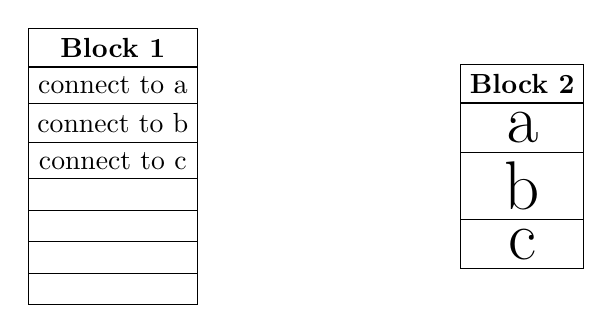
\begin{tikzpicture}[
  grow=right,    
  level 1/.style={sibling distance=3.5cm,level distance=5.2cm},
  edge from parent/.style={draw=white},
]

\node[name=block1, rectangle split, rectangle split parts=8, draw=black]
  { \textbf{Block 1}
    \nodepart{second} connect to a
    \nodepart{third} connect to b
    \nodepart{fourth} connect to c
  }
  child {
    node[name=block2, rectangle split, rectangle split parts=4, draw=black]
     {  \textbf{Block 2}
        \nodepart{second} \Huge{a}
        \nodepart{third} \Huge{b}
        \nodepart{fourth} \Huge{c}
    }
};
\end{tikzpicture}


%C
\tikzset{
    table nodes/.style={
        rectangle,
        draw=black,
        align=center,
        minimum height=7mm,
        text depth=0.5ex,
        text height=2ex,
        inner xsep=0pt,
        outer sep=0pt
    },      
    table/.style={
        matrix of nodes,
        row sep=-\pgflinewidth,
        column sep=-\pgflinewidth,
        nodes={
            table nodes
        },
        execute at empty cell={\node[draw=none]{};}
    }
}
\begin{tikzpicture}

\matrix (first) [table,text width=7mm,name=table]
{
A   & B & C & D\\
E   &   &   & F\\
};
\node[draw,fit=(table-2-2)(table-2-3),table nodes]{F};


\matrix (first) [table,text width=7mm,name=table]
{
A   & B & C & D\\
E   &   &   & F\\
};
\node[draw,fit=(table-2-2)(table-2-3),table nodes]{F};

\end{tikzpicture}


\end{document}